\subsection{Deskripsi dan Analisis Usulan}

\subsubsection{Deskripsi Usulan}

Usulan penelitian ini adalah merancang dan mengimplementasikan aplikasi Jatidiri berbasis mobile sebagai media penyajian tes psikologi dengan memanfaatkan framework Flutter dan metode Prototype. Aplikasi Jatidiri dikembangkan berdasarkan desain antarmuka pengguna (UI/UX) yang telah dibuat menggunakan Figma, kemudian diterjemahkan ke dalam komponen Flutter agar dapat dijalankan pada perangkat mobile berbasis Android.

Aplikasi ini menyediakan berbagai fitur utama, yaitu halaman beranda (Home), halaman tes psikologi yang berisi berbagai jenis tes seperti tes kecerdasan, tes kecemasan, tes bakat, tes stres, dan tes potensi, serta halaman komunitas yang memungkinkan pengguna berinteraksi. Fokus utama pengembangan adalah implementasi antarmuka aplikasi yang interaktif, responsif, dan sesuai dengan desain yang telah ditetapkan.

Dengan menerapkan metode Prototype, pengembangan aplikasi dilakukan secara iteratif melalui pembuatan purwarupa awal, evaluasi, dan penyempurnaan berdasarkan umpan balik dari pembimbing atau pemangku kepentingan, hingga diperoleh aplikasi yang sesuai dengan kebutuhan.


\subsubsection{Analisis Usulan}

Analisis usulan dilakukan untuk menilai kelayakan dan relevansi solusi yang diusulkan terhadap permasalahan yang ada. Permasalahan utama yang dihadapi adalah bagaimana menerjemahkan desain UI dari Figma ke dalam aplikasi Flutter yang fungsional dan konsisten, serta bagaimana memastikan bahwa antarmuka aplikasi dapat digunakan dengan mudah oleh pengguna.

Usulan pengembangan aplikasi Jatidiri dinilai layak karena didukung oleh teknologi yang matang, yaitu Flutter sebagai framework lintas platform, Dart sebagai bahasa pemrograman, serta Figma sebagai alat desain UI. Metode Prototype dipilih karena sesuai untuk proyek yang berfokus pada iterasi desain dan penyempurnaan antarmuka secara berkelanjutan.

Dari sisi manfaat, usulan ini diharapkan dapat menghasilkan aplikasi mobile yang tidak hanya fungsional tetapi juga memiliki kualitas antarmuka yang baik, sehingga meningkatkan pengalaman pengguna dalam mengakses tes psikologi secara digital.


\subsection{Analisis Kebutuhan Fungsional dan Non-Fungsional}

\subsubsection{Analisis Kebutuhan Fungsional}

Kebutuhan fungsional menggambarkan fungsi-fungsi yang harus dimiliki oleh sistem agar dapat berjalan sesuai tujuan. Adapun kebutuhan fungsional aplikasi Jatidiri adalah sebagai berikut:

1. Sistem dapat menampilkan halaman beranda (Home) sebagai halaman utama aplikasi.

2. Sistem dapat menampilkan daftar tes psikologi yang tersedia.

3. Sistem memungkinkan pengguna memilih dan mengerjakan tes psikologi.

4. Sistem dapat menampilkan hasil tes kepada pengguna.

5. Sistem menyediakan halaman komunitas untuk interaksi pengguna.

6. Sistem dapat menampilkan informasi profil pengguna.

7. Sistem dapat menyimpan dan menampilkan riwayat hasil tes pengguna.


\subsubsection{Analisis Kebutuhan Non-Fungsional}

Kebutuhan non-fungsional menggambarkan kualitas dan batasan sistem agar dapat beroperasi secara optimal. Kebutuhan non-fungsional aplikasi Jatidiri meliputi:

1. Kinerja (Performance): Aplikasi harus berjalan dengan responsif dan waktu muat halaman tidak lebih dari beberapa detik.

2. Usability: Antarmuka harus mudah digunakan dan dipahami oleh pengguna awam.

3. Reliability: Aplikasi harus stabil dan tidak sering mengalami crash.

4. Compatibility: Aplikasi dapat berjalan pada berbagai perangkat Android dengan ukuran layar yang berbeda.

5. Security: Data pengguna harus disimpan dan diproses secara aman.

6. Maintainability: Kode aplikasi harus terstruktur dan mudah dikembangkan lebih lanjut.


\subsection{Metodologi}

\subsubsection{Metode yang Digunakan}

\begin{figure}[htbp]
    \centering
    % Metode Yang Digunakan
    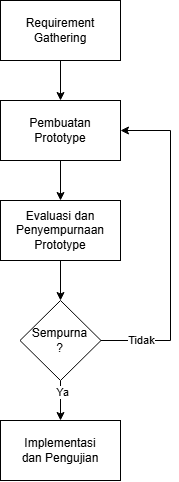
\includegraphics[width=0.3\textwidth]{figures/metode.png}
    \caption{Metode Prototype}
    \label{fig:Metode Prototype}
\end{figure}

Metodologi yang digunakan dalam pengembangan aplikasi Jatidiri adalah metode Prototype, yang menekankan pada pengembangan sistem secara iteratif melalui pembuatan purwarupa (prototype) dan penyempurnaan berulang berdasarkan umpan balik dari pengguna atau pemangku kepentingan. Metode ini memungkinkan pengembang untuk memperoleh pemahaman yang lebih baik mengenai kebutuhan pengguna serta menyesuaikan desain antarmuka sebelum aplikasi diimplementasikan secara final. Pendekatan ini sangat sesuai untuk pengembangan aplikasi yang berfokus pada antarmuka pengguna (UI/UX), seperti pada aplikasi Jatidiri yang dikembangkan berdasarkan desain Figma dan diimplementasikan menggunakan framework Flutter. Tahapan utama dalam metode Prototype meliputi:


1. Requirements Gathering

Fase pertama adalah pengumpulan kebutuhan (requirement gathering), yang bertujuan untuk memahami kebutuhan fungsional dan nonfungsional aplikasi, khususnya terkait struktur halaman, navigasi, dan elemen antarmuka pengguna. Pada tahap ini, kebutuhan sistem diperoleh dari desain UI/UX yang telah dibuat menggunakan Figma serta diskusi dengan pembimbing atau pemangku kepentingan. Fase ini sangat penting karena menjadi dasar dalam pengembangan prototype yang sesuai dengan harapan pengguna. Menurut Santos et al. (2020), metode Prototype sangat efektif ketika kebutuhan sistem belum sepenuhnya terdefinisi secara rinci di awal dan memungkinkan klarifikasi kebutuhan dilakukan secara bertahap selama proses pengembangan. Selain itu, keterlibatan pemangku kepentingan sejak tahap awal berkontribusi terhadap peningkatan kesesuaian antara sistem yang dikembangkan dengan kebutuhan pengguna (Preece et al., 2021).


2. Pembuatan Prototype

Tahap pembuatan prototype berfokus pada pengembangan versi awal aplikasi yang merepresentasikan tampilan dan alur interaksi pengguna. Pada penelitian ini, prototype diwujudkan melalui implementasi desain antarmuka dari Figma ke dalam komponen Flutter. Prototype yang dihasilkan mencakup struktur halaman utama, halaman tes, serta halaman komunitas. Tahap ini bersifat iteratif, sehingga prototype dapat dimodifikasi dan disempurnakan berdasarkan masukan yang diperoleh. Penelitian menunjukkan bahwa penggunaan prototype secara iteratif dapat meningkatkan kualitas desain antarmuka dan mengurangi risiko kesalahan desain yang signifikan pada tahap akhir pengembangan (Silva et al., 2021). Pendekatan ini juga memungkinkan pengembang untuk menguji kesesuaian tampilan dan interaksi sebelum aplikasi dikembangkan secara penuh.


3. Evaluasi dan Penyempurnaan Prototype

Prototype yang telah dibuat kemudian dievaluasi untuk menilai kesesuaian antara desain, fungsionalitas, dan pengalaman pengguna. Evaluasi dilakukan melalui pengujian internal serta umpan balik dari pihak terkait, yang kemudian digunakan sebagai dasar untuk melakukan penyempurnaan prototype. Tahap ini memungkinkan identifikasi dini terhadap masalah usability, inkonsistensi desain, maupun kekurangan fungsionalitas sebelum implementasi final dilakukan. Menurut Assila et al. (2020), evaluasi usability pada tahap prototyping sangat penting untuk meningkatkan kualitas interaksi pengguna dan meminimalkan kebutuhan perbaikan besar pada tahap akhir. Proses evaluasi dan penyempurnaan ini dilakukan secara berulang hingga prototype dianggap memenuhi kebutuhan pengguna dan siap untuk diimplementasikan secara final.


4. Implementasi dan Pengujian

Tahap terakhir adalah implementasi prototype yang telah disempurnakan menjadi aplikasi mobile yang siap digunakan. Pada tahap ini, seluruh antarmuka aplikasi Jatidiri diimplementasikan menggunakan framework Flutter dan bahasa pemrograman Dart. Setelah implementasi selesai, dilakukan pengujian menggunakan metode black box testing untuk memastikan bahwa setiap fitur dan tampilan antarmuka berfungsi sesuai dengan kebutuhan dan desain yang telah ditetapkan. Pengujian ini bertujuan untuk mengidentifikasi kesalahan fungsional serta memastikan stabilitas aplikasi sebelum digunakan oleh pengguna. Pengujian pada tahap akhir merupakan bagian penting dalam metode Prototype untuk menjamin kualitas aplikasi yang dihasilkan (Alshamrani \& Bahattab, 2022).


\subsubsection{Diagram BPMN}

Untuk menggambarkan alur interaksi antara pengguna dan sistem dalam aplikasi Jatidiri, digunakan pemodelan proses bisnis dengan Business Process Model and Notation (BPMN). Diagram BPMN ini disusun menggunakan dua lane utama dalam satu pool, yaitu Pengguna dan Sistem (Aplikasi Jatidiri), guna memisahkan aktivitas yang dilakukan oleh pengguna dan respons yang diberikan oleh sistem.

Proses dimulai pada lane Sistem (Aplikasi Jatidiri) dengan Start Event, yang merepresentasikan dimulainya proses ketika aplikasi menampilkan Splash Screen. Selanjutnya, sistem menampilkan halaman Walkthrough sebagai pengenalan awal fitur aplikasi. Setelah itu, pengguna berinteraksi dengan sistem melalui pilihan Login atau Register yang dimodelkan menggunakan Exclusive Gateway (XOR).

Setelah pengguna berhasil melewati tahap autentikasi, sistem menampilkan halaman Survei yang harus diisi pengguna sebelum masuk ke halaman Home. Pada halaman Home, pengguna dapat memilih antara menu Tes atau Komunitas, yang juga dimodelkan menggunakan Exclusive Gateway. Jika pengguna memilih Tes, sistem akan menampilkan daftar tes, detail tes, dan halaman soal secara berulang hingga tes selesai. Jika pengguna memilih Komunitas, sistem menampilkan halaman komunitas sebelum pengguna kembali ke Home.

\begin{figure}[htbp]
    \centering
    % Diagram BPMN
    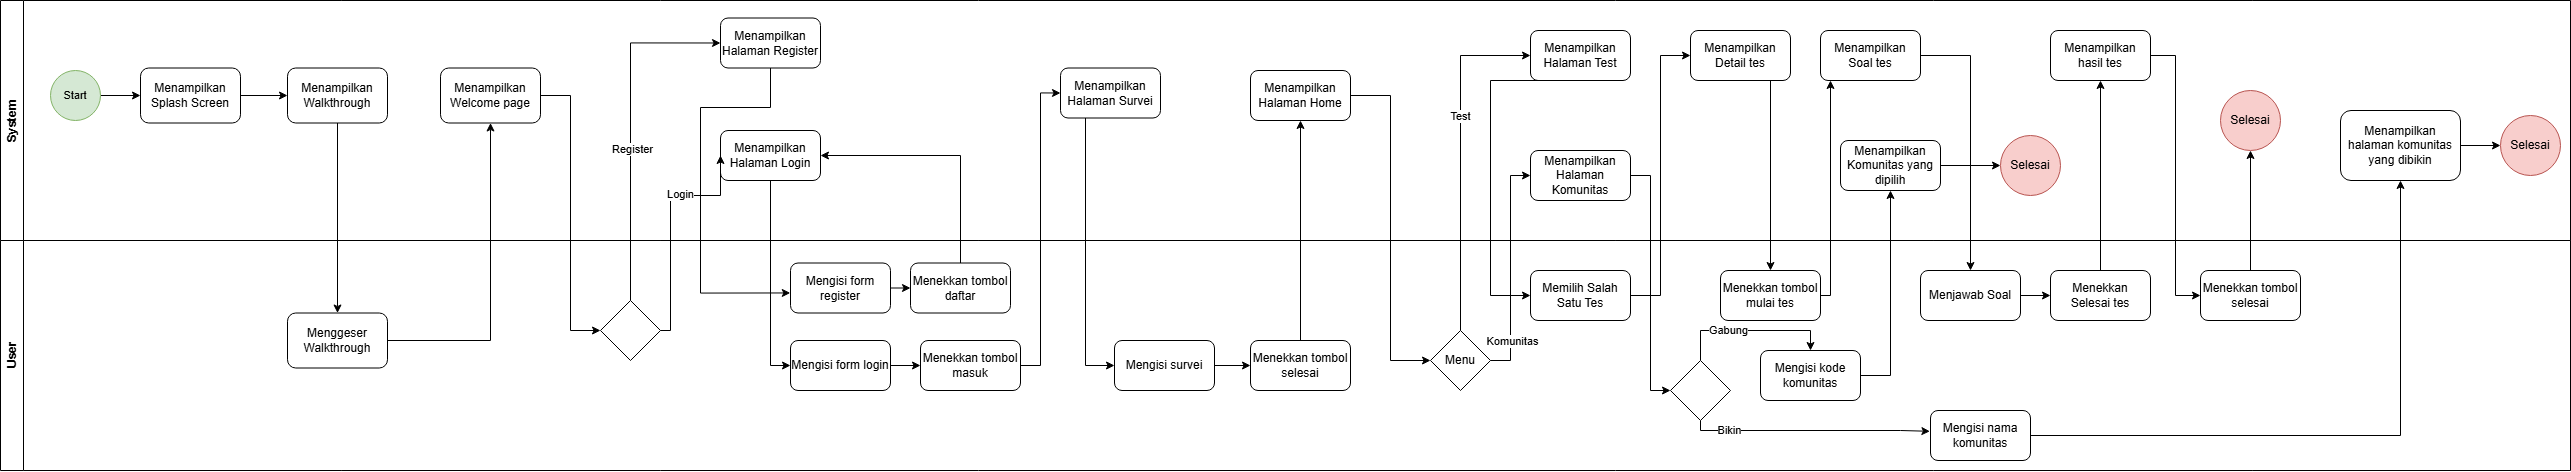
\includegraphics[width=1\textwidth]{figures/bpmn.png}
    \caption{Diagram BPMN}
    \label{fig:Diagram BPMN}
\end{figure}
